\subsection{Random Projection}\label{subsec:random_projection}


% cosine distance
cosine distance makes sense in spaces that have dimensions, including euclidean spaces and discrete versions of euclidean spaces \cite[95]{leskovec_rajaraman_ullman_2014}

calculate the cosine distance by first computing the cosine of the angle, and then applying the arc-cosine function to translate an angle in the 0-180 degree range \cite[95]{leskovec_rajaraman_ullman_2014}
cosine distance between two points is the angle that the angle of that vectors to those points make; this angle is in the range 0 to 180 degrees, regardless of the dimensionality of the Space

\begin{definition}[Cosine Distance]
    Given two vectors $p_1$ and $p_2$, the cosine distance $\theta(p_1, p_2)$ is the dot product of $p_1$ and $p_2$ divided by their euclidean distances from the origin ($L_2$-norm):
    \begin{equation}
        \theta(\bm{p}_1, \bm{p}_2) = \text{cos}^{-1} \bigg( \frac{\bm{x}_1 \cdot \bm{x}_2}{||\bm{p}_1|| \: ||\bm{p}_2||} \Bigg).
    \end{equation}
\end{definition}

$\theta$ can be divided by $\pi$ to have a distance in the range $[0,1]$.

\begin{definition}[Cosine Similarity]
    Opposed to the cosine distance, the cosine similarity is defined as
    \begin{equation}
        1- \theta(\bm{p}_1, \bm{p}_2)
    \end{equation}
\end{definition}



Introduced in \cite{charikar2002similarity}
Given a message $\bm{x} \in A = \{x \in \mathbb{R}^d : 0 \leq x \leq 1 \}$ and a randomly selected hyperplane defined as $\bm{M}=(a_{ij}) \in \mathbb{R}^{d \times k}$ where $a \sim \mathcal{N}(0, I)$, a \textit{gaussian random projection (GRP)} aims to (\RomanNumeralCaps{1}) reduce the dimensionality from $d$ to $l$ dimensions and (\RomanNumeralCaps{2}) provide a binary encoding by first projecting $\bm{x}$ onto $\bm{M}$ and subsequently applying the sign function to each element of the result, i.e. :

\begin{align*}
    h(\bm{x}) = [h(\bm{x}, a_1), \dots, h(\bm{x}, a_k)] \text{ with } h(\bm{x}, a) = sign(\bm{x}^Ta) \\
    \text{with } sign(x) = \Biggl\{ \begin{array}{lc}
        0 & \text{if } x < 0 \\
        1 & \text{if } x \geq 0
    \end{array}.
\end{align*}

The resulting digest is a binary vector $h(\bm{x}) = \bm{u} \in B = \{0, 1\}^l$ that is commonly used as bucket index for storing $\bm{x}$ in a hash table. For any two messages $\bm{x}_1, \bm{x}_2$, the probability of being hashed to the same bucket increases with a decreasing distance, which is given by the angular distance as

\begin{equation}\label{eq:rp_proba}
    P[h(\bm{x}_1) = h(\bm{x}_2)] = 1 - \frac{\theta(\bm{x}_1, \bm{x}_2)}{\pi}
\end{equation}

\begin{figure}
    \centering
    \begin{subfigure}[b]{0.45\textwidth}
        \centering
        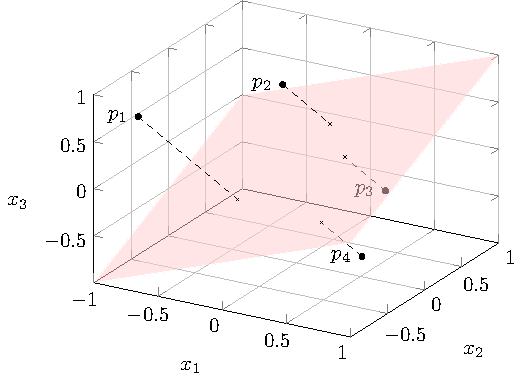
\includegraphics[width=\textwidth]{tikz/random_projection.pdf}
        \caption{Illustration of a random hyperplane (red) partitioning the space.}
        \label{subfig:rp_3d}
    \end{subfigure}
    \hfill
    \begin{subfigure}[b]{0.45\textwidth}
        \centering
        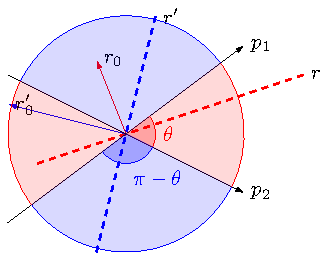
\includegraphics[width=\textwidth]{tikz/random_hyperplane_2d.pdf}
        \caption{Visual Proof of claim in equation \ref{eq:rp_proba}}
        \label{subfig:rp_2d}
    \end{subfigure}
    \caption{}
    \label{fig:random_projection}
\end{figure}

Consider Figure \ref{subfig:rp_2d}, where two vectors $p_1$ and $p_2$, regardless of their dimensionality, define a plane and an angle $\theta$ in this plane.

Pick a hyperplane (actually the normal vector to the hyperplane; hyperplane $v$ is the set of points whose dot product with $v$ is 0)

Hyperplane intersects the plane that is spanned by two vectors $p_1$ and $p_2$ in a line

vector $r_0$ that is normal to the hyperplane represented by the red dashed line; $p_1$ and $p_2$ are on different sides of the hyperplane, thus the projections given by $\langle p_1, r_0 \rangle$ and  $\langle p_2, r_0 \rangle$ will have different signs

vector $r'_0$ that is normal to the hyperplane represented by the blue dashed line;  both $\langle p_1, r'_0 \rangle$ and  $\langle p_2, r'_0 \rangle$ will have the same sign

All angles between the intersection line of the random hyperplane and the plane spanned by $p_1$ and $p_2$ are equally likely. Thus, the probability that the hyperplane looks like the red line is $\theta / \pi$ and like the blue line otherwise.

random projections is a $(R, cR, (1-R/\pi), (1-cR/\pi))$-sensitive family for any $R$ and $cR$. As already explained in Section \ref{subsec:locality-sensitive-hashes}, such a family can be amplified as desired.